%% Manuscript for Computers & Security (Elsevier) -- elsarticle class.
%% Every experimental number comes from tables/numbers.tex, produced by make_figures.py.
\documentclass[preprint,12pt,authoryear]{elsarticle}
\usepackage{amsmath,amssymb,amsthm}
\usepackage{graphicx,booktabs,multirow}
\usepackage[hidelinks]{hyperref}
\usepackage{xcolor}
\newtheorem{theorem}{Theorem}
\newtheorem{proposition}{Proposition}
\newtheorem{definition}{Definition}
% auto-generated by make_figures.py -- do not edit by hand
\newcommand{\HiddenCats}{cryptominer, exploit, p2p\mbox{-}worm, pua, rootkit and trojan\mbox{-}gamethief}
\newcommand{\NHiddenCats}{6}
\newcommand{\NSeeds}{3}
\newcommand{\SeedsNoun}{seeds}
\newcommand{\NMutable}{2{,}284}
\newcommand{\NMonotone}{15}
\newcommand{\NFeatures}{2{,}381}
\newcommand{\MutablePct}{96}
\newcommand{\NCategories}{14}
\newcommand{\NFamilies}{353}
\newcommand{\LgbmAcc}{99.53}
\newcommand{\MlpAcc}{99.23}
\newcommand{\MlpGroupEvadeOne}{93.9}
\newcommand{\AblOneCleanAcc}{97.88}
\newcommand{\AblOneCertR}{92.5}
\newcommand{\AblOneCertRtwo}{84.0}
\newcommand{\AblViolations}{0}
\newcommand{\TrainEps}{0.05}
\newcommand{\CrownAsymCert}{98.2}
\newcommand{\CrownAsymCertUnc}{96.9}
\newcommand{\CrownAsymAcc}{98.71}
\newcommand{\CrownSymCert}{97.9}
\newcommand{\CrownSymCertUnc}{96.2}
\newcommand{\CrownSymCertTen}{44.2}
\newcommand{\CrownSymCertTenUnc}{9.7}
\newcommand{\CrownAsymCertTen}{38.4}
\newcommand{\CrownSymCertStd}{0.2}
\newcommand{\CrownAsymCertStd}{0.3}
\newcommand{\CrownSymCertTenStd}{4.6}
\newcommand{\CrownAsymCertTenStd}{7.5}
\newcommand{\AsymGainSeeds}{in every seed}
\newcommand{\AsymLossTenSeeds}{in every seed}
\newcommand{\IbpCert}{97.3}
\newcommand{\CrownSymAcc}{99.33}
\newcommand{\CrownSymFpr}{0.64}
\newcommand{\CrownAsymFpr}{2.02}
\newcommand{\StdAccSmall}{99.13}
\newcommand{\AblTwoCertR}{94.7}
\newcommand{\AblTwoCleanAcc}{98.77}
\newcommand{\AblThreeCertR}{94.9}
\newcommand{\AblThreeCleanAcc}{99.24}
\newcommand{\AblOneEmpR}{93.9}
\newcommand{\AblOneEmpRtwo}{84.1}
\newcommand{\RsSigmaMax}{1.0}
\newcommand{\RsIsoAccMax}{99.3}
\newcommand{\RsSubAccMax}{99.4}
\newcommand{\NCert}{10{,}000}
\newcommand{\NCertPoints}{1{,}000}
\newcommand{\StdCert}{12.6}
\newcommand{\PgdAtCert}{6.9}
\newcommand{\RsSigma}{0.5}
\newcommand{\RsIsoAcc}{99.2}
\newcommand{\RsSubAcc}{99.1}
\newcommand{\RsSubHalf}{99.1}
\newcommand{\RsIsoHalf}{99.0}
\newcommand{\CTViolations}{0}
\newcommand{\AtkEps}{0.1}
\newcommand{\MlpPgdCon}{79.9}
\newcommand{\MlpPgdUnc}{89.2}
\newcommand{\AtPgdCon}{1.9}

% auto-generated by tools/make_temporal.py -- do not edit by hand
\newcommand{\TmpTestStart}{2020-06-30}
\newcommand{\TmpTestEnd}{2020-09-30}
\newcommand{\TmpTrainEnd}{2020-05-27}
\newcommand{\TmpCertEps}{0.05}
\newcommand{\TmpAblTprDrop}{15.6}
\newcommand{\TmpAblCertDrop}{19.3}
\newcommand{\TmpAblDropStd}{3.3}
\newcommand{\TmpAblCertVsClean}{more than}
\newcommand{\TmpAblTprDropStd}{3.1}
\newcommand{\TmpAblCertDropStd}{1.2}
\newcommand{\TmpAblGap}{3.7}
\newcommand{\TmpAblGapRatio}{1.1}
\newcommand{\TmpAblDropRatio}{1.2}
\newcommand{\TmpAblDropRatioInt}{1}
\newcommand{\TmpCrownTprDrop}{1.9}
\newcommand{\TmpCrownCertDrop}{9.3}
\newcommand{\TmpCrownDropStd}{1.8}
\newcommand{\TmpCrownCertVsClean}{more than}
\newcommand{\TmpCrownTprDropStd}{0.3}
\newcommand{\TmpCrownCertDropStd}{1.8}
\newcommand{\TmpCrownGap}{7.4}
\newcommand{\TmpCrownGapRatio}{4.1}
\newcommand{\TmpCrownDropRatio}{4.8}
\newcommand{\TmpCrownDropRatioInt}{5}
\newcommand{\TmpMlpFprRand}{0.74}
\newcommand{\TmpMlpFprTemp}{0.19}
\newcommand{\TmpCrownFprRand}{0.64}
\newcommand{\TmpCrownFprTemp}{0.04}
\newcommand{\TmpFprDropModels}{every model}
\newcommand{\TmpMlpAccRand}{99.23}
\newcommand{\TmpMlpAccTemp}{97.43}
\newcommand{\TmpCrownAccRand}{99.33}
\newcommand{\TmpCrownAccTemp}{98.64}
\newcommand{\TmpMlpAccLoss}{1.8}
\newcommand{\TmpCrownAccLoss}{0.7}
\newcommand{\TmpAccLossStd}{0.5}
\newcommand{\TmpCrownVsMlpAccSentence}{CROWN-IBP also loses less clean accuracy than the standard MLP (\TmpCrownAccLoss{} vs.\ \TmpMlpAccLoss{} points), a gap larger than their combined seed-to-seed standard deviation (\TmpAccLossStd{} points).}
\newcommand{\TmpMalShareRand}{42.6}
\newcommand{\TmpMalShareTemp}{50.4}
\newcommand{\TmpMalShareCmp}{larger}
\newcommand{\TmpMlpTprLoss}{4.1}
\newcommand{\TmpCrownTprLoss}{1.9}
\newcommand{\TmpTprLossStd}{0.9}
\newcommand{\TmpCrownVsMlpSentence}{Under drift, CROWN-IBP loses less malware detection than the standard MLP (\TmpCrownTprLoss{} vs.\ \TmpMlpTprLoss{} points of TPR), a gap larger than their combined seed-to-seed standard deviation (\TmpTprLossStd{} points).}
\newcommand{\TmpAblTwoTprDrop}{8.1}
\newcommand{\TmpAblTwoTprDropStd}{0.2}
\newcommand{\TmpAblTwoCertDrop}{17.5}
\newcommand{\TmpAblTwoCertDropStd}{4.1}
\newcommand{\TmpAblThreeTprDrop}{2.0}
\newcommand{\TmpAblThreeTprDropStd}{0.1}
\newcommand{\TmpAblThreeCertDrop}{14.3}
\newcommand{\TmpAblThreeCertDropStd}{1.7}
\newcommand{\TmpAblKTprCmp}{less than}
\newcommand{\TmpAblKCertCmp}{less than}
\newcommand{\TmpAblCertDropMin}{14.3}
\newcommand{\TmpAblCertDropMax}{19.3}

\journal{Computers \& Security}

\begin{document}
\begin{frontmatter}
\title{Certified Robustness of Machine-Learning Malware Detectors in Constrained {PE} Feature Space: Group-Ablation Certificates and Constraint-Aware Certified Training}

\author[inst1]{Ababil Hossain Fahad\corref{cor1}}
\ead{fahad@lamppost.org.bd}
\cortext[cor1]{Corresponding author}
\affiliation[inst1]{organization={\textcolor{red}{[Department, Institution]}}, city={Dhaka}, country={Bangladesh}}

\begin{abstract}
Machine-learning malware detectors are now central to endpoint security pipelines, yet they remain sensitive to gradient-based adversarial perturbations. Existing certified defenses such as randomized smoothing and interval bound propagation were designed for images: they treat every input dimension as equally changeable and describe the attacker by a small norm ball, whereas Portable Executable (PE) features are partly immutable, partly increase-only, and are rewritten group by group by real evasion tools. We make three contributions, evaluated on a stratified 30,000-sample subset of BODMAS (12,773 malware, 17,227 benign; \NCategories{} malware categories and \NFamilies{} families) represented by 2,381-dimensional LIEF/EMBER features. (i) We formalise a constraint-aware feature-space threat model in which only \NMutable{} features are attacker-mutable and \NMonotone{} can only increase, and show that a single transplanted feature group evades a \MlpAcc\%-accurate neural detector on \MlpGroupEvadeOne\% of attacked malware. (ii) We introduce feature-group ablation smoothing, a deterministic certificate against arbitrary modification of up to $r$ semantic feature groups; with single-group views it certifies \AblOneCertR\% of malware against any one-group modification and \AblOneCertRtwo\% against two, with no counter-example found by the attack. (iii) We propose constraint-aware CROWN-IBP training, which propagates bounds only through the reachable region of feature space; at $\epsilon=\TrainEps$ it certifies \CrownSymCert\% of malware (\CrownSymCertUnc\% when bounded over the unconstrained box) at \CrownSymAcc\% clean accuracy, versus \StdCert\% for a standard network. Requiring robustness only for malware does not pay off: its certified-detection gain at $\epsilon=\TrainEps$ (\CrownAsymCert\% vs.\ \CrownSymCert\%) is within seed-to-seed variation, and it raises the false-positive rate from \CrownSymFpr\% to \CrownAsymFpr\%.
\end{abstract}

\begin{keyword}
Malware detection \sep Adversarial machine learning \sep Certified robustness \sep Randomized smoothing \sep Interval bound propagation \sep Portable Executable
\end{keyword}
\end{frontmatter}

%% ===================================================================================
\section{Introduction}
Static machine-learning detectors classify Windows PE files from features extracted without execution, such as byte histograms, string statistics, header fields and hashed import tables \citep{anderson2018ember,gibert2020rise}. They are fast and generalise to unseen variants, but they inherit the adversarial fragility of neural networks \citep{szegedy2014intriguing,goodfellow2015explaining}: small, functionality-preserving edits to a binary can flip the decision \citep{grosse2017adversarial,kolosnjaji2018adversarial,demetrio2021exemples,pierazzi2020problemspace}.

Empirical defenses such as adversarial training \citep{madry2018towards,aldujaili2018adversarial} raise the cost of known attacks but give no guarantee against stronger ones. Certified defenses provide a proof that no perturbation inside a threat set changes the prediction. The two dominant families, randomized smoothing \citep{lecuyer2019certified,cohen2019certified} and bound propagation \citep{gowal2018ibp,zhang2018crown,zhang2020crownibp}, were developed for images, where every pixel is equally mutable and an $\ell_p$ ball is a reasonable proxy for imperceptibility. PE feature vectors violate both assumptions: (a) many features (e.g.\ machine type, subsystem, data-directory sizes) cannot be changed without breaking the executable, (b) many others can only grow under append-only edits, and (c) features come in semantically coherent groups whose scales differ by orders of magnitude. Applying image-style certificates uniformly over all 2,381 dimensions therefore wastes certification budget on impossible perturbations, and a norm ball cannot express the edits that matter most in practice, such as rebuilding an entire import table.

Certified robustness for malware has so far focused on raw-byte models, certifying against byte patches or insertions via (de)randomized smoothing over byte windows \citep{saha2024drsm,gibert2024certified} or randomized deletion \citep{huang2023rsdel}, and on architectures that are robust by construction \citep{incer2018monotonic,gimenez2025erdalt}. Structured feature-space detectors, which remain the industry standard, lack certificates that exploit their structure. This paper fills that gap with three contributions:
\begin{enumerate}
\item \textbf{C1 -- Constraint-aware threat model and attacks.} We annotate each EMBER feature as immutable, mutable, or monotone (increase-only), define the reachable region as their intersection with the empirical feature domain, and implement FGSM/PGD and a group-transplant attack inside it. The model over-approximates functionality-preserving problem-space edits, so certificates proved against it are sound for the real attacker.
\item \textbf{C2 -- Feature-group ablation certificates and subspace smoothing.} We adapt de-randomized ablation \citep{levine2020ablation,levine2020patch} from pixels to the nine semantic EMBER groups, giving a deterministic certificate against \emph{arbitrary} changes to up to $r$ groups, and we restrict Gaussian smoothing to the mutable subspace.
\item \textbf{C3 -- Constraint-aware certified training.} We propagate IBP/CROWN bounds through the constrained box instead of the full $\ell_\infty$ ball. We also evaluate an asymmetric variant that requires robustness only for the malware class, since benign authors have no incentive to evade; it yields a negative result (Section~\ref{sec:ct}).
\end{enumerate}
All experiments use BODMAS \citep{yang2021bodmas}, and every reported number is generated by released scripts.

%% ===================================================================================
\section{Related work}
\textbf{Evasion of static detectors.} Feature-space attacks on malware detectors date back at least to \citet{grosse2017adversarial}; problem-space attacks that edit real binaries (header manipulation, section injection, padding) are surveyed by \citet{demetrio2021exemples}, and \citet{pierazzi2020problemspace} formalise the gap between feature-space and problem-space adversaries. Our threat model follows their principle that only realisable transformations should be counted.

\textbf{Empirical defenses.} Adversarial training \citep{madry2018towards} has been applied to binary-encoded malware \citep{aldujaili2018adversarial}. Monotonic classifiers \citep{incer2018monotonic} are robust by construction to addition-only attacks; \citet{chen2020pdf} train PDF classifiers with verified robustness properties.

\textbf{Certified defenses.} Randomized smoothing gives probabilistic $\ell_2$ certificates \citep{cohen2019certified,lecuyer2019certified,salman2019provably}; de-randomized ablation gives deterministic $\ell_0$ and patch certificates \citep{levine2020ablation,levine2020patch}. IBP \citep{gowal2018ibp}, CROWN \citep{zhang2018crown} and CROWN-IBP \citep{zhang2020crownibp} bound network outputs over input boxes and can be used both to verify and to train. For malware, DRSM \citep{saha2024drsm} and \citet{gibert2024certified} certify raw-byte detectors against contiguous patches, RS-Del \citep{huang2023rsdel} certifies against edit-distance perturbations of byte sequences, and ERDALT \citep{gimenez2025erdalt} builds detectors that are robust by design. Concurrent work \citep{giri2026towards} smooths an EMBER-feature detector with Gaussian noise and random group ablation during training and certifies an $\ell_2$ radius, but it does not certify against modification of feature groups or model which features an attacker can change, which is our focus.

%% ===================================================================================
\section{Threat model}\label{sec:threat}
Let $x\in\mathbb{R}^{d}$, $d=2381$, be the EMBER feature vector after a per-feature signed-log and z-score transform $\phi$. Because $\phi$ is strictly increasing per coordinate, ``feature $i$ can only increase'' is preserved in the transformed space.

\begin{definition}[Feature annotation]
Each coordinate $i$ is \emph{immutable} ($i\notin\mathcal{M}$), \emph{mutable} ($i\in\mathcal{M}$) or \emph{monotone} ($i\in\mathcal{N}\subseteq\mathcal{M}$, increase-only). We take as mutable the byte and byte-entropy histograms, string statistics, section, import and export groups, file size and virtual size, the import/export counts in the general block and the COFF timestamp, i.e.\ everything reachable by appending data, adding strings, adding a section or import, or editing the timestamp. Counts and sizes are monotone. Header fields other than the timestamp and the data-directory table are immutable. This yields $|\mathcal{M}|=\NMutable$ and $|\mathcal{N}|=\NMonotone$.
\end{definition}

\begin{definition}[Constrained $\ell_\infty$ region]
For budget $\epsilon$ the reachable box is $B_\epsilon(x)=\prod_i[\ell_i,u_i]$ with $\ell_i=u_i=x_i$ for $i\notin\mathcal{M}$, $\ell_i=x_i$, $u_i=x_i+\epsilon$ for $i\in\mathcal{N}$, $[\ell_i,u_i]=[x_i-\epsilon,x_i+\epsilon]$ otherwise, intersected with the training-set range of feature $i$ (extended to contain $x_i$).
\end{definition}

\begin{definition}[Group threat]
EMBER features form $G=9$ groups (byte histogram, byte-entropy histogram, strings, general+timestamp, static header, section, imports, exports, data directories). An $r$-group adversary may replace \emph{all} features of any $r$ mutable groups by arbitrary values. This $\ell_0$-over-groups model needs no norm or scale assumption and directly matches edits such as ``add a section'' or ``rebuild the import table''.
\end{definition}

Only malware is attacked: the adversary wants a malicious file labelled benign. All the above sets contain every realisable edit we consider, so a certificate against them is sound, if conservative, for the real attacker.

%% ===================================================================================
\section{Methods}
\subsection{C1: constrained gradient attacks}
FGSM and PGD \citep{goodfellow2015explaining,madry2018towards} maximise the cross-entropy of the true label with the projection $\Pi_{B_\epsilon(x)}$ applied after every step: clip to $[-\epsilon,\epsilon]$, zero the step on immutable features, clip monotone steps at zero and clip to the feature domain. The \emph{group-transplant} attack greedily copies whole mutable groups from benign donor samples, choosing at each step the group and donor that most reduce the malware score, up to $r$ groups.

\subsection{C2a: feature-group ablation certificate}
For a keep-size $k$ let $\mathcal{V}_k$ be all $\binom{G}{k}$ subsets of groups. A base network $h(x\odot m_S, \mathbf{1}_S)$ sees the features of the kept groups $S$ (others set to the training mean) and a $G$-bit indicator of which groups are kept; it is trained on random subsets of size $k$. The smoothed classifier votes over all views: $n_c(x)=|\{S\in\mathcal{V}_k: h_S(x)=c\}|$ and $g(x)=\arg\max_c n_c(x)$. Following the argument of \citet{levine2020patch} for de-randomized patch certificates, we bound how many views a modification of $r$ groups can reach.
\begin{theorem}\label{thm:abl}
Let $\Delta_r=\binom{G}{k}-\binom{G-r}{k}$. If $n_y(x)-n_{c}(x)>2\Delta_r$ for every $c\neq y$, then $g(x')=y$ for every $x'$ that differs from $x$ only within at most $r$ groups.
\end{theorem}
\begin{proof}
A view $S$ is unaffected unless it keeps at least one modified group. The number of $k$-subsets that avoid a fixed set of $r$ groups is $\binom{G-r}{k}$, so at most $\Delta_r$ views can change their vote. Each changed vote lowers $n_y$ by at most one and raises some $n_c$ by at most one, so $n_y(x')-n_c(x')\ge n_y(x)-n_c(x)-2\Delta_r>0$.
\end{proof}
The certificate is deterministic and exact to compute ($\binom{G}{k}\le 84$ forward passes for $k\le3$), and it holds for any values written into the modified groups, not only small ones.

\subsection{C2b: subspace randomized smoothing}
Isotropic smoothing \citep{cohen2019certified} adds $\mathcal{N}(0,\sigma^2 I)$ to all features. We add noise only on $\mathcal{M}$: $\eta\sim\mathcal{N}(0,\sigma^2 P_\mathcal{M})$, with $P_\mathcal{M}$ the coordinate projection. For perturbations $\delta$ supported on $\mathcal{M}$, the immutable coordinates of $x$ and $x+\delta$ coincide, so Cohen et al.'s theorem applied in $\mathbb{R}^{|\mathcal{M}|}$ gives the radius $R=\sigma\,\Phi^{-1}(\underline{p_A})$, where $\underline{p_A}$ is a one-sided Clopper--Pearson lower bound \citep{clopper1934} on the top-class probability. The base network is trained with the same noise distribution.

\subsection{C3: constraint-aware certified training}
For a ReLU network with logits $z$, let $m(x)=z_y(x)-z_{1-y}(x)$. IBP \citep{gowal2018ibp} and CROWN \citep{zhang2018crown} give sound lower bounds $\underline{m}$ over any input box. We evaluate them over $B_\epsilon(x)$ rather than the full $\ell_\infty$ ball:
\begin{proposition}
For any sound box-bounding method, $B_\epsilon(x)\subseteq\{x':\|x'-x\|_\infty\le\epsilon\}$ implies that every point certified under the unconstrained box is certified under $B_\epsilon(x)$.
\end{proposition}
Training minimises $\kappa\,\mathrm{CE}(z(x),y)+(1-\kappa)\,\mathrm{softplus}(-\underline{m}(x))$ with the CROWN-IBP mixture $\underline{m}=\beta\,\underline{m}_{\text{CROWN}}+(1-\beta)\,\underline{m}_{\text{IBP}}$ \citep{zhang2020crownibp}; $\epsilon$ ramps linearly from 0 after a clean warm-up while $\kappa$ goes $1\to0.5$ and $\beta$ goes $1\to0$. We also evaluate an \emph{asymmetric} variant, in which the robust term is applied only to malware samples and benign samples keep the clean loss; Section~\ref{sec:ct} reports it as a negative result. At test time a point is certified if $\max(\underline{m}_{\text{IBP}},\underline{m}_{\text{CROWN}})>0$.

%% ===================================================================================
\section{Experimental setup}
\textbf{Data.} From the 134,435 BODMAS samples \citep{yang2021bodmas} we draw 12,773 malware (stratified by category, keeping at least five samples of every category) and 17,227 benign samples, and split them 70/10/20, stratified by category. A temporal split \citep{pendlebury2019tesseract} is evaluated in Section~\ref{sec:temporal}. Features are transformed by signed $\log(1+|x|)$ and z-scored with training statistics.

\textbf{Models.} LightGBM \citep{ke2017lightgbm} serves as the EMBER reference detector. Neural detectors are ReLU MLPs (2381--512--256--2 for attacks, smoothing and ablation; 2381--256--256--2 for certified training), trained with Adam and a cosine schedule. PGD adversarial training uses the constrained region with $\epsilon=0.1$ and 10 steps. All hyperparameters were set before the experiments, except that after a preliminary run we extended the smoothing grid to $\sigma=1.0$ to probe larger noise; all values tried are reported. The validation split was not used for tuning or model selection.

\textbf{Evaluation.} We report accuracy, F1, true-positive rate (TPR, malware detected), false-positive rate and AUC on the test split; under attack we report the malware TPR that survives the attack, and for certificates the \emph{certified TPR}, the fraction of test malware that is correctly classified and certified. Smoothing uses $n_0=100$ selection and $n$ certification samples with $\alpha=10^{-3}$. Results are averaged over \NSeeds{} \SeedsNoun{} (mean $\pm$ std).

%% ===================================================================================
\section{Results}\label{sec:results}
%% Results narrative. Numbers are macros from tables/numbers.tex; re-check every qualitative
%% sentence (marked %CHECK) after the final full run, since directions can change.

\subsection{Clean detection}
Table~\ref{tab:clean} lists clean performance. LightGBM, the EMBER reference model, reaches \LgbmAcc\% accuracy and the standard MLP \MlpAcc\%. Most certifiable models cost little or no clean accuracy: the symmetric CROWN-IBP network reaches \CrownSymAcc\% (standard network of the same size: \StdAccSmall\%). The clearest cost is group ablation with single-group views ($k=1$, \AblOneCleanAcc\%), which loses more than one point against the standard MLP; larger keep sizes recover most of it ($k=3$: \AblThreeCleanAcc\%). %CHECK

\begin{table}[t]\centering\small
\caption{Clean test performance (mean $\pm$ std over \NSeeds{} \SeedsNoun{}).}\label{tab:clean}
\resizebox{\linewidth}{!}{\begin{tabular}{lccccc}
\toprule
Model & Acc. (\%) & F1 (\%) & TPR (\%) & FPR (\%) & AUC \\
\midrule
LightGBM (EMBER baseline) & 99.53$\pm$0.05 & 99.45$\pm$0.06 & 99.39$\pm$0.11 & 0.36$\pm$0.01 & 0.9998$\pm$0.0001 \\
MLP (standard) & 99.23$\pm$0.17 & 99.10$\pm$0.20 & 99.21$\pm$0.20 & 0.74$\pm$0.15 & 0.9985$\pm$0.0004 \\
MLP + PGD-AT & 99.34$\pm$0.11 & 99.22$\pm$0.13 & 99.27$\pm$0.15 & 0.61$\pm$0.09 & 0.9994$\pm$0.0003 \\
Group ablation, $k$=1 & 97.88$\pm$0.19 & 97.48$\pm$0.23 & 95.92$\pm$0.27 & 0.66$\pm$0.13 & 0.9972$\pm$0.0007 \\
Group ablation, $k$=2 & 98.77$\pm$0.05 & 98.56$\pm$0.06 & 98.40$\pm$0.18 & 0.95$\pm$0.12 & 0.9991$\pm$0.0002 \\
Group ablation, $k$=3 & 99.24$\pm$0.11 & 99.11$\pm$0.13 & 99.04$\pm$0.07 & 0.61$\pm$0.14 & 0.9994$\pm$0.0004 \\
IBP ($\epsilon$=0.05) & 99.37$\pm$0.16 & 99.26$\pm$0.19 & 99.35$\pm$0.16 & 0.61$\pm$0.17 & 0.9989$\pm$0.0004 \\
CROWN-IBP ($\epsilon$=0.05) & 99.33$\pm$0.17 & 99.21$\pm$0.20 & 99.28$\pm$0.24 & 0.64$\pm$0.13 & 0.9990$\pm$0.0004 \\
CROWN-IBP (asym.) ($\epsilon$=0.05) & 98.71$\pm$0.08 & 98.51$\pm$0.09 & 99.70$\pm$0.10 & 2.02$\pm$0.11 & 0.9950$\pm$0.0008 \\
\bottomrule
\end{tabular}}
\end{table}

\subsection{C1: constrained attacks}
Figure~\ref{fig:attacks} and Table~\ref{tab:attacks} show the malware detection rate that survives FGSM and PGD. Restricting the attacker to the reachable region weakens every attack: at $\epsilon=\AtkEps$, PGD evades the standard MLP on \MlpPgdCon\% of malware under constraints versus \MlpPgdUnc\% without them, so unconstrained evaluations overstate the threat. PGD adversarial training at $\epsilon=0.1$ reduces constrained evasion at the same budget to \AtPgdCon\%; its protection degrades beyond the training budget and is gone by $\epsilon=0.5$ (Table~\ref{tab:attacks}). %CHECK The group-transplant attack is far more damaging: copying a single feature group from a benign file evades the standard MLP on \MlpGroupEvadeOne\% of attacked malware (Fig.~\ref{fig:group}, grey). This motivates certificates against group-level edits rather than small norm balls.

\begin{figure}[t]\centering
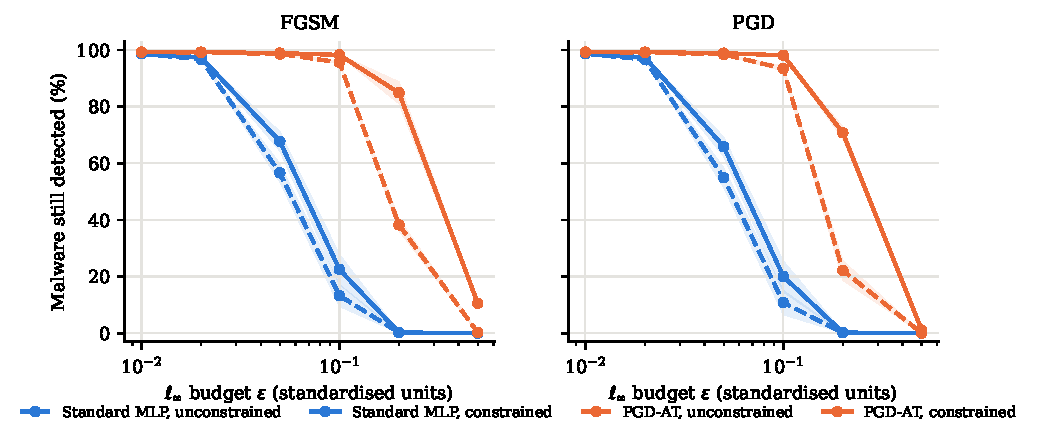
\includegraphics[width=\linewidth]{figures/fig_attacks.pdf}
\caption{Malware still detected under FGSM and PGD as the $\ell_\infty$ budget grows. Dashed: unconstrained attacker; solid: constrained (C1) attacker.}\label{fig:attacks}
\end{figure}

\begin{table}[t]\centering\small
\caption{Malware detection rate (\%) under PGD.}\label{tab:attacks}
\resizebox{\linewidth}{!}{\begin{tabular}{lrrrr}
\toprule
Detector & $r=0$ & $r=1$ & $r=2$ & $r=3$ \\
\midrule
LightGBM (all features) & 88.5 & 0.0 & 0.0 & 0.0 \\
LightGBM, monotonic & 88.6 & 0.0 & 0.0 & 0.0 \\
MLP 2381--512--256--2 & 83.3 & 0.2 & 0.0 & 0.0 \\
MLP 2381--256--256--2 & 82.3 & 0.2 & 0.0 & 0.0 \\
PGD-AT on $B_\epsilon$ & 83.5 & 0.3 & 0.0 & 0.0 \\
Group ablation, MLP views, main & 74.1 & 49.9 & 0.0 & 0.0 \\
Group ablation, MLP views, second & 69.8 & 26.1 & 0.0 & 0.0 \\
Group ablation, MLP views, EMBER groups & 60.8 & 0.0 & 0.0 & 0.0 \\
Group ablation, LightGBM views, main & 83.4 & 62.6 & 0.0 & 0.0 \\
Group ablation, LightGBM views, second & 78.8 & 37.0 & 0.0 & 0.0 \\
CROWN-IBP, uniform ball & 82.3 & 0.0 & 0.0 & 0.0 \\
CROWN-IBP, constrained box & 84.5 & 0.2 & 0.0 & 0.0 \\
CROWN-IBP, edit-aware & 81.5 & 2.0 & 0.1 & 0.0 \\
Giri et al., re-implementation & 82.3 & 0.7 & 0.0 & 0.0 \\
\bottomrule
\end{tabular}
% malware detected (%) under the group-transplant attack in the main partition's groups; mean over 5 seeds; 500 malware, 10 donors}
\end{table}

\subsection{C2a: feature-group ablation certificates}
Table~\ref{tab:group} and Fig.~\ref{fig:group} report certified detection as a function of the number $r$ of modified groups. Keep-size $k$ trades clean accuracy for certifiable $r$: with $k=1$ (nine single-group views) the detector certifies \AblOneCertR\% of malware against any change to one group and \AblOneCertRtwo\% against two, at \AblOneCleanAcc\% clean accuracy; $k=2$ certifies \AblTwoCertR\% at $r=1$ with \AblTwoCleanAcc\% accuracy; $k=3$ certifies \AblThreeCertR\% at $r=1$ with \AblThreeCleanAcc\% accuracy but nothing at $r\geq2$, as Theorem~\ref{thm:abl} predicts ($2\Delta_2=98$ exceeds the 84 views). The greedy group-transplant attack against the $k=1$ detector leaves \AblOneEmpR\% and \AblOneEmpRtwo\% of malware detected at $r=1,2$, close to the certified values, so the certificate is nearly tight. Across all runs the attack never evaded a certified sample (\AblViolations{} violations), as required by soundness.

\begin{figure}[t]\centering
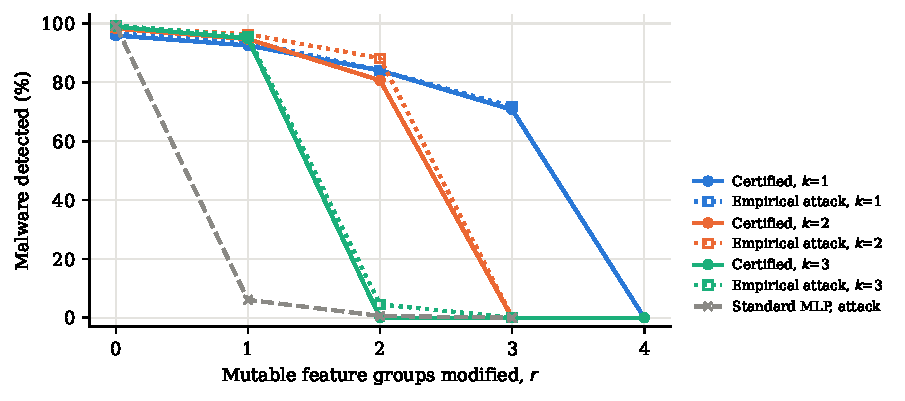
\includegraphics[width=0.88\linewidth]{figures/fig_group_cert.pdf}
\caption{Certified malware detection (solid) and detection under the group-transplant attack (dotted) versus the number of modified groups. Grey: undefended MLP.}\label{fig:group}
\end{figure}

\begin{table}[t]\centering\small
\caption{Certified malware detection (\%) of group-ablation smoothing against $r$ modified groups.}\label{tab:group}
\resizebox{\linewidth}{!}{\begin{tabular}{lrrrrrrrr}
\toprule
 & \multicolumn{3}{c}{$r$ needed} & \multicolumn{5}{c}{Certified detection (\%)} \\
\cmidrule(lr){2-4}\cmidrule(lr){5-9}
Edit type & main & second & EMBER & main, MLP & main, LightGBM & second, MLP & second, LightGBM & EMBER, MLP \\
\midrule
E1 overlay append & 1 & 1 & 4 & 36.6 & 55.1 & 57.7 & 64.4 & 0.0 \\
E2 string padding & 1 & 1 & 4 & 36.6 & 55.1 & 57.7 & 64.4 & 0.0 \\
E3 section injection & 2 & 2 & 6 & 0.0 & 0.0 & 42.1 & 52.4 & 0.0 \\
E4 import addition & 3 & 3 & 7 & 0.0 & 0.0 & 18.2 & 32.2 & 0.0 \\
E5 timestamp & 1 & 1 & 3 & 36.6 & 55.1 & 57.7 & 64.4 & 27.0 \\
E6 section renaming & 2 & 2 & 4 & 0.0 & 0.0 & 42.1 & 52.4 & 0.0 \\
E7 checksum, DOS header & 1 & 1 & 3 & 36.6 & 55.1 & 57.7 & 64.4 & 27.0 \\
E8 signature/debug strip & 2 & 3 & 6 & 0.0 & 0.0 & 18.2 & 32.2 & 0.0 \\
E10 header versions & 1 & 2 & 3 & 36.6 & 55.1 & 42.1 & 52.4 & 27.0 \\
\midrule
Mean over the nine types &  &  &  & 20.3\,$\pm$\,3.9 & 30.6\,$\pm$\,5.2 & 43.7\,$\pm$\,5.2 & 53.2\,$\pm$\,8.6 & 9.0\,$\pm$\,2.3 \\
Clean accuracy &  &  &  & 88.5\,$\pm$\,3.3 & 92.8\,$\pm$\,2.4 & 86.0\,$\pm$\,3.6 & 90.8\,$\pm$\,5.1 & 83.0\,$\pm$\,2.7 \\
Views; largest certifiable $r$ &  &  &  & 10; 1 & 10; 1 & 7; 3 & 7; 3 & 9; 4 \\
\bottomrule
\end{tabular}
% family split, 5 seeds; main = aligned5 k=2, second = aligned7 k=1, EMBER = 9 groups k=1}
\end{table}

\subsection{C2b: randomized smoothing}
Contrary to the common assumption that smoothing collapses clean accuracy on PE features, Gaussian smoothing in standardised feature space keeps clean accuracy high: at $\sigma=\RsSigmaMax$ it is \RsIsoAccMax\% (isotropic) and \RsSubAccMax\% (subspace) on the \NCertPoints{} certified test points. %CHECK
Restricting noise to the mutable subspace gives at most a small change (\RsSubHalf\% vs.\ \RsIsoHalf\% certified at $R=0.5$, $\sigma=\RsSigma$), because \MutablePct\% of the features are mutable: the subspace removes little noise. %CHECK
The sharp drop of each curve in Fig.~\ref{fig:smoothing} is the sampling ceiling $\sigma\Phi^{-1}(\underline{p_A})$ for $n=\NCert$ samples, not a property of the classifier. Smoothing radii in standardised $\ell_2$ units are also hard to relate to real edits, which is why we treat this certificate as a baseline rather than a headline result.

\begin{figure}[t]\centering
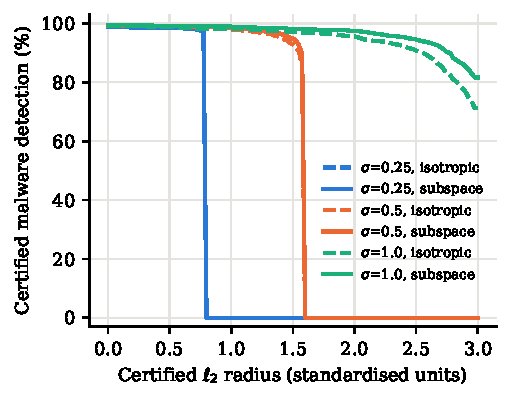
\includegraphics[width=0.62\linewidth]{figures/fig_smoothing.pdf}
\caption{Certified malware detection of Gaussian smoothing versus $\ell_2$ radius; dashed: noise on all features, solid: noise only on mutable features.}\label{fig:smoothing}
\end{figure}

\begin{table}[t]\centering\small
\caption{Randomized smoothing: clean accuracy and certified malware detection (\%) at several radii.}\label{tab:smoothing}
\resizebox{\linewidth}{!}{\begin{tabular}{llccccc}
\toprule
$\sigma$ & Noise & Clean acc. (\%) & $R\geq$0.0 & $R\geq$0.25 & $R\geq$0.5 & $R\geq$1.0 \\
\midrule
0.25 & isotropic & 99.1$\pm$0.4 & 99.1 & 99.0 & 98.6 & 0.0 \\
0.25 & subspace & 99.1$\pm$0.3 & 98.9 & 98.7 & 98.5 & 0.0 \\
0.5 & isotropic & 99.2$\pm$0.2 & 99.4 & 99.3 & 99.0 & 98.0 \\
0.5 & subspace & 99.1$\pm$0.3 & 99.2 & 99.1 & 99.1 & 98.4 \\
1.0 & isotropic & 99.3$\pm$0.4 & 99.3 & 99.2 & 98.9 & 98.0 \\
1.0 & subspace & 99.4$\pm$0.2 & 99.4 & 99.3 & 99.3 & 98.9 \\
\bottomrule
\end{tabular}}
\end{table}

\subsection{C3: constraint-aware certified training}\label{sec:ct}
Figure~\ref{fig:ct} and Table~\ref{tab:ct} show certified malware detection under the constrained $\ell_\infty$ threat. Standard and PGD-trained networks are rarely certifiable at the training budget ($\epsilon=\TrainEps$: \StdCert\% and \PgdAtCert\%), although PGD-AT resists the attack empirically. IBP and CROWN-IBP training raise certified detection to \IbpCert\% and \CrownSymCert\% at no measurable cost in clean accuracy. Bounding over the constrained box instead of the full ball certifies more samples, and the gain grows with the budget: \CrownSymCert\% vs.\ \CrownSymCertUnc\% at $\epsilon=\TrainEps$ and \CrownSymCertTen\% vs.\ \CrownSymCertTenUnc\% at $\epsilon=0.1$. %CHECK
Asymmetric training does not pay off. At $\epsilon=\TrainEps$ it certifies \CrownAsymCert$\pm$\CrownAsymCertStd\% of malware versus \CrownSymCert$\pm$\CrownSymCertStd\% for symmetric CROWN-IBP, a gain within seed-to-seed variation (though positive \AsymGainSeeds); at $\epsilon=0.1$ it certifies less (\CrownAsymCertTen$\pm$\CrownAsymCertTenStd\% vs.\ \CrownSymCertTen$\pm$\CrownSymCertTenStd\%, lower \AsymLossTenSeeds); and it raises the false-positive rate from \CrownSymFpr\% to \CrownAsymFpr\%: making only malware robust pushes the decision boundary into benign territory. In deployment, where false positives are costly, symmetric CROWN-IBP is the better operating point. %CHECK
No sample certified by bound propagation was ever evaded by PGD (\CTViolations{} violations).

\begin{figure}[t]\centering
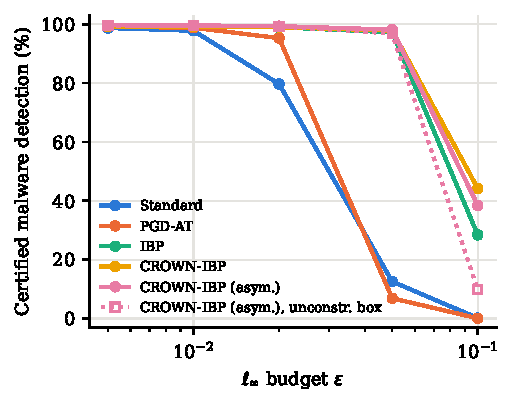
\includegraphics[width=0.62\linewidth]{figures/fig_certified_training.pdf}
\caption{Certified malware detection versus $\ell_\infty$ budget (constrained box), for networks with the same 2381--256--256--2 architecture. Dotted: asymmetric CROWN-IBP certified over the unconstrained box.}\label{fig:ct}
\end{figure}

\begin{table}[t]\centering\small
\caption{Certified malware detection (\%) under the constrained $\ell_\infty$ threat; last column: certified samples evaded by PGD (must be 0).}\label{tab:ct}
\resizebox{\linewidth}{!}{\begin{tabular}{lrrrrrrrr}
\toprule
 & & & \multicolumn{5}{c}{Certified over $T_f(1)$ (\%)} & \\
\cmidrule(lr){4-8}
CROWN-IBP training & Acc. & FPR & content & section & import & strip & mean & $B_\epsilon$, $\epsilon=0.05$ \\
\midrule
Standard MLP & 91.7 & 0.6 & 0.0 & 0.0 & 0.0 & 0.0 & 0.0\,$\pm$\,0.0 & 3.6 \\
PGD-AT & 92.7 & 0.4 & 0.0 & 0.0 & 0.0 & 0.0 & 0.0\,$\pm$\,0.0 & 1.7 \\
Uniform ball, $\epsilon=0.1$ (tuned) & 92.2 & 0.4 & 0.0 & 0.0 & 0.0 & 0.1 & 0.0\,$\pm$\,0.0 & 72.6 \\
Constrained box, $\epsilon=0.1$ & 93.0 & 0.4 & 0.0 & 0.0 & 0.0 & 0.0 & 0.0\,$\pm$\,0.0 & 73.1 \\
Edit-aware & 91.4 & 1.2 & 40.7 & 66.8 & 40.2 & 76.3 & 56.0\,$\pm$\,7.0 & 71.0 \\
Uniform ball, $\epsilon=1$ (sweep) & 89.9 & 6.5 & 72.5 & 32.6 & 0.0 & 84.2 & 47.3\,$\pm$\,17.6 & -- \\
\bottomrule
\end{tabular}
% family split, 5 seeds (sweep row: results_eps_sweep); networks 2381--256--256--2}
\end{table}

\subsection{Per-category robustness}
Figure~\ref{fig:cat} breaks certified detection down by malware category, averaged over the \NSeeds{} seeds' test splits. Large categories (trojan, worm, backdoor) are certified at high rates by every method, trojans being the lowest of the three, while bound-propagation certificates are more uniform across categories than the group certificate. The group certificate is lowest on file-infecting viruses, plausibly because an infected host is mostly benign content so few single-group views vote malware. This observation remains tentative: each test split holds fewer than ten viruses, and even across all seeds the number of distinct viruses tested (shown in the figure) is small. Information stealers and viruses are the two weakest categories for every method. %CHECK

\begin{figure}[t]\centering
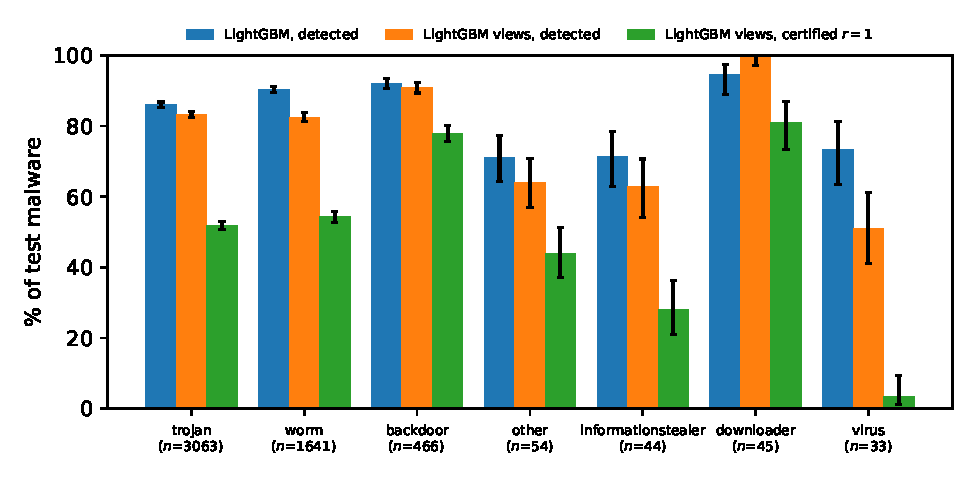
\includegraphics[width=0.72\linewidth]{figures/fig_per_category.pdf}
\caption{Certified malware detection (\%) per category, averaged over the \NSeeds{} seeds' test splits ($n$ = distinct test files across all seeds). Not shown, for having fewer than three test samples per seed on average: \HiddenCats.}\label{fig:cat}
\end{figure}

\subsection{Robustness under temporal drift}\label{sec:temporal}
Following the temporal-split principle of \citet{pendlebury2019tesseract}, in which every training file precedes every test file, we also train on files up to \TmpTrainEnd{} and test on the later window \TmpTestStart{} to \TmpTestEnd{} (Tables~\ref{tab:temporal-clean} and~\ref{tab:temporal-cert}). We measure drift by malware detection (TPR) rather than accuracy: the false-positive rate drops for \TmpFprDropModels{} on the temporal window (standard MLP: \TmpMlpFprRand\% to \TmpMlpFprTemp\%; CROWN-IBP: \TmpCrownFprRand\% to \TmpCrownFprTemp\%), which inflates accuracy, and the temporal test window holds a \TmpMalShareCmp{} share of malware (\TmpMalShareTemp\% vs.\ \TmpMalShareRand\%), which changes accuracy as well. For CROWN-IBP, clean detection falls by \TmpCrownTprDrop$\pm$\TmpCrownTprDropStd{} points and certified detection at $\epsilon=\TmpCertEps$ by \TmpCrownCertDrop$\pm$\TmpCrownCertDropStd{}, roughly \TmpCrownDropRatioInt{} times as much; the gap is \TmpCrownGapRatio{} times their combined standard deviation. For group ablation ($k=1$), clean detection falls by \TmpAblTprDrop$\pm$\TmpAblTprDropStd{} points and certified detection at $r=1$ by \TmpAblCertDrop$\pm$\TmpAblCertDropStd{}; the gap of \TmpAblGap{} points is about one combined standard deviation (\TmpAblDropStd{}), so we do not claim it as significant. Across keep sizes, $k=3$ drifts less than $k=1$ in both clean and certified detection (\TmpAblThreeTprDrop$\pm$\TmpAblThreeTprDropStd{} vs.\ \TmpAblTprDrop$\pm$\TmpAblTprDropStd{} points of clean detection; \TmpAblThreeCertDrop$\pm$\TmpAblThreeCertDropStd{} vs.\ \TmpAblCertDrop$\pm$\TmpAblCertDropStd{} points of certified detection at $r=1$); $k=2$ lies between on average, with high variance in certified detection (\TmpAblTwoCertDrop$\pm$\TmpAblTwoCertDropStd{} points). \TmpCrownVsMlpSentence{} \TmpCrownVsMlpAccSentence{} %CHECK

\begin{table}[t]\centering\small
\caption{Clean test performance (\%) under the random and the temporal split (mean $\pm$ std over \NSeeds{} \SeedsNoun{}). The temporal split uses one fixed test window (\TmpTestStart{} to \TmpTestEnd{}), so its $\pm$ reflects training randomness only; values without $\pm$ are identical across seeds.}\label{tab:temporal-clean}
\resizebox{\linewidth}{!}{\begin{tabular}{lcccccc}
\toprule
 & \multicolumn{3}{c}{Random split} & \multicolumn{3}{c}{Temporal split} \\
\cmidrule(lr){2-4}\cmidrule(lr){5-7}
Model & Acc. & TPR & FPR & Acc. & TPR & FPR \\
\midrule
LightGBM & 99.53$\pm$0.05 & 99.39$\pm$0.11 & 0.36$\pm$0.01 & 99.52 & 99.11 & 0.07 \\
MLP (standard) & 99.23$\pm$0.17 & 99.21$\pm$0.20 & 0.74$\pm$0.15 & 97.43$\pm$0.40 & 95.09$\pm$0.82 & 0.19$\pm$0.03 \\
MLP + PGD-AT & 99.34$\pm$0.11 & 99.27$\pm$0.15 & 0.61$\pm$0.09 & 98.96$\pm$0.09 & 98.03$\pm$0.18 & 0.09$\pm$0.02 \\
Group ablation, $k$=1 & 97.88$\pm$0.19 & 95.92$\pm$0.27 & 0.66$\pm$0.13 & 90.06$\pm$1.55 & 80.36$\pm$3.06 & 0.08$\pm$0.02 \\
Group ablation, $k$=2 & 98.77$\pm$0.05 & 98.40$\pm$0.18 & 0.95$\pm$0.12 & 95.04$\pm$0.03 & 90.28$\pm$0.05 & 0.12$\pm$0.02 \\
Group ablation, $k$=3 & 99.24$\pm$0.11 & 99.04$\pm$0.07 & 0.61$\pm$0.14 & 98.44$\pm$0.04 & 96.99$\pm$0.07 & 0.09$\pm$0.02 \\
CROWN-IBP ($\epsilon$=0.05) & 99.33$\pm$0.17 & 99.28$\pm$0.24 & 0.64$\pm$0.13 & 98.64$\pm$0.08 & 97.35$\pm$0.17 & 0.04$\pm$0.02 \\
\bottomrule
\end{tabular}}
\end{table}

\begin{table}[t]\centering\small
\caption{Certified malware detection (\%) under the random and the temporal split (mean $\pm$ std over \NSeeds{} \SeedsNoun{}), and its drop (random minus temporal), whose $\pm$ combines the standard deviations of both splits. In the text, differences between drops are judged against the combined seed-to-seed standard deviation, which is conservative (assumes independence).}\label{tab:temporal-cert}
\resizebox{\linewidth}{!}{\begin{tabular}{llccc}
\toprule
Model & Certificate & Random split & Temporal split & Drop \\
\midrule
Group ablation, $k$=1 & $r$=1 & 92.5$\pm$0.7 & 73.2$\pm$0.9 & 19.3$\pm$1.2 \\
Group ablation, $k$=1 & $r$=2 & 84.0$\pm$0.4 & 61.1$\pm$2.9 & 22.9$\pm$2.9 \\
Group ablation, $k$=2 & $r$=1 & 94.7$\pm$0.2 & 77.2$\pm$4.1 & 17.5$\pm$4.1 \\
Group ablation, $k$=2 & $r$=2 & 80.7$\pm$0.4 & 56.2$\pm$0.9 & 24.5$\pm$1.0 \\
Group ablation, $k$=3 & $r$=1 & 94.9$\pm$0.1 & 80.6$\pm$1.7 & 14.3$\pm$1.7 \\
Group ablation, $k$=3 & $r$=2 & 0.0 & 0.0 & 0.0 \\
CROWN-IBP & $\epsilon$=0.05 & 97.9$\pm$0.2 & 88.6$\pm$1.8 & 9.3$\pm$1.8 \\
\bottomrule
\end{tabular}}
\end{table}


%% ===================================================================================
\section{Discussion and limitations}
\textbf{Feature space versus problem space.} All certificates are stated in feature space. Because our sets over-approximate realisable edits, they are sound for those edits, but they may be loose: a certificate against $r=1$ group covers any change to the import table, including changes that no real linker could produce. Conversely, attacks that alter immutable features by rewriting the binary (e.g.\ repacking) fall outside the model; this is a deliberate scoping choice shared with prior work \citep{pierazzi2020problemspace,demetrio2021exemples}.

\textbf{Choice of norm units.} $\ell_\infty$ and $\ell_2$ budgets are expressed in standardised units, which are not directly interpretable in bytes. The group certificate avoids this issue entirely, which is one reason we regard it as the most practically meaningful of the three. That judgement holds for a fixed data distribution only: under temporal drift the group certificate degrades more than CROWN-IBP, its certified detection at $r=1$ falling by \TmpAblCertDropMin{}--\TmpAblCertDropMax{} points across keep sizes against \TmpCrownCertDrop{} for CROWN-IBP (Section~\ref{sec:temporal}).

\textbf{Concept drift.} Our temporal evaluation (Section~\ref{sec:temporal}) covers a single test window (\TmpTestStart{} to \TmpTestEnd{}) after the training period, and certified detection measured on a random split need not carry over to later samples at the same rate. On that window, CROWN-IBP's certified detection falls by \TmpCrownCertDrop{} points against \TmpCrownTprDrop{} for its clean detection, roughly \TmpCrownDropRatioInt{} times as much, so certificates should be recomputed as malware evolves rather than assumed to persist. Longer horizons and retraining strategies, as studied by \citet{pendlebury2019tesseract}, remain to be evaluated.

%% ===================================================================================
\section{Conclusion}
We showed that structure-blind certified defenses are a poor fit for PE feature vectors, and that exploiting three simple facts (some features are immutable, some only grow, and features come in semantic groups) yields certificates that are both meaningful and cheap. Feature-group ablation in particular gives deterministic, norm-free guarantees against modification of whole feature groups, the kind of edit real evasion tools perform. Under temporal drift, however, both certificates lose ground: the group certificate's certified detection at $r=1$ falls by \TmpAblCertDropMin{}--\TmpAblCertDropMax{} points depending on the keep size, and CROWN-IBP's by \TmpCrownCertDrop{} points against \TmpCrownTprDrop{} for its clean detection, roughly \TmpCrownDropRatioInt{} times as much, so certificates should be recomputed as malware evolves.

\section*{CRediT authorship contribution statement}
\textbf{Ababil Hossain Fahad:} Conceptualization, Methodology, Software, Investigation, Writing -- original draft.

\section*{Declaration of competing interest}
The author declares no competing financial interests or personal relationships that could have appeared to influence the work reported in this paper.

\section*{Data availability}
BODMAS is publicly available from its authors. Code to reproduce all experiments, figures and tables will be released upon publication.

\section*{Declaration of generative AI use}
\textcolor{red}{[Elsevier requires a statement if AI tools were used in writing; describe your use here.]}

\bibliographystyle{elsarticle-harv}
\bibliography{refs}
\end{document}
